\chapter{Introduction}\label{chapter:intro}

  \section{Membranes for Aqueous Separations}
  
  %BJC: limiting to pressure driven aqueous membrane separations (so I don't have to get into electrodialysis, gas separations, dialysis etc.)
  Pressure driven membrane processes have become an increasingly useful tool for
  performing aqueous separations.
  \begin{itemize}
    \item Untreated water can be a very complex solution with particles ranging
    in size from microns down to nanometers
    \item Sediment, bacteria, algae, proteins, small organic molecules, and ions
    are all common components of aqueous streams.
  \end{itemize}
  
  % TFC membranes review -- "Composite reverse osmosis and nanofiltration membranes"
  \noindent Membrane design is completely dependent on the target particle separation. 
  \begin{itemize}
    \item Membranes are classified based on the size of the particle they reject.
    \item Microfiltration membranes contain pores with diameters ranging from 100-10000 nm.
    They can separate large particles like bacteria and protozoa.~\cite{ma_functionalized_2014}
    \item Ultrafiltration membranes have pore diameters of about 5-500 nm and are useful for the 
    separation of sugars, proteins, viruses and colloidal materials.~\cite{yanful_ultrafiltration_2009}
    \item Nanofiltration have pores on the order of 1 nm in diameter and can be used for the separation
    of small organic molecules and charged species.~\cite{van_der_bruggen_review_2003}
    \item Reverse osmosis membranes are dense amorphous polymers with no explicit pores. Their
    dense polymer architecture rejects all solutes to a high degree except for water making
    them useful for separating hydrated ions from water.~\cite{warsinger_review_2018}
    \item We have summarized the uses of different classes of membrane 
    technologies in Figure~\ref{fig:size_regimes}.
    \item To deal with complex aqueous streams, and to prevent excessive membrane fouling, 
    these technologies are often used in series, removing larger particles first.~\cite{goosen_fouling_2005}
  \end{itemize}
  
  \begin{figure}
  \centering
  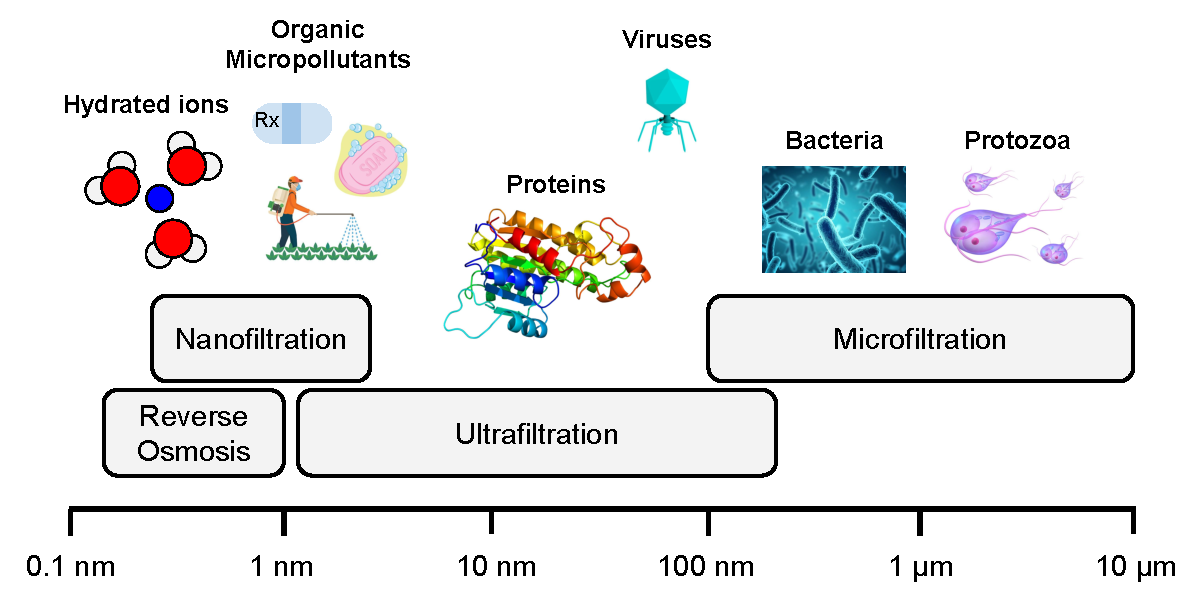
\includegraphics[width=\textwidth]{figs/membrane_separation_size_regimes.pdf}
  \caption{}\label{fig:size_regimes}
  \end{figure}
  
  \noindent Membrane permeation is the result of a chemical potential gradient, $\frac{d\mu_i}{dx}$.
  \begin{itemize}
	  \item The flux of component $i$ is proportional to this gradient:
	  \begin{equation}
	    J_i = -L_i \frac{d\mu_i}{dx}
	  \end{equation}
	  where $L_i$ is a coefficient of proportionality.~\cite{wijmans_solution-diffusion_1995}
	  \item Chemical potential gradients can be induced by concentration, pressure, 
	  temperature and electromotive forces.
	  \item We will limit our discussion to concentration and pressure gradients.
  \end{itemize}
  
  % This follows the discussion of werber_material_2016
  For pressure driven membrane processes, water flux through both porous and 
  amorphous membranes can be described by
  \begin{equation}
  J_w = A(\Delta P - \Delta \pi_m)
  \end{equation}
  where $J_w$ is volumetric water flux, $A$ is the water permeability coefficient,
  $\Delta P$ is the applied hydraulic pressure and $\Delta \pi_m$ is the 
  trans-membrane osmotic pressure difference. The water permeability coefficient
  is dependent on how one models flow through the membrane.
  
  In porous membrane architectures, water flux is modeled as laminar flow through 
  cylindrical pores.
  \begin{itemize}
    \item The derivation follows Hagen-Poiseuille flow with inclusion of morphological
    characteristics:
    \begin{equation}
      A = \frac{\varepsilon r_p^2}{8\mu\delta_m}
    \end{equation}
    where $\varepsilon$ is the surface porosity, $r_p$ the pore radius, $\delta_m$ the
    membrane thickness, and $\mu$ the solution viscosity.
    \item Separation is typically characterized in terms of solute rejection, $R$. 
    \begin{equation}
      R = 1 - \frac{c_p}{c_f}
    \end{equation}
    where $c_p$ and $c_f$ are the concentrations of the rejected species in
    the permeate and feed respectively.
    \item Solutes with radii smaller than the pore will be rejected. A distribution of 
    pore sizes prevents perfect rejection.
  \end{itemize}
  
  In amorphous membranes, water and solute flux are modeled using the solution-diffusion 
  model.
  \begin{itemize}
    \item It is hypothesized that water and solute molecules partition into the
    membrane and diffuse across the polymer matrix due to a chemical potential
    gradient and then desorb into the permeate.
    \item The product of a component's solubility and diffusivity is commonly
    referred to as its permeability, $P$.~\cite{wijmans_solution-diffusion_1995}
    \item $P$ is an intrinsic material property and is thus independent of membrane
    thickness.  % BJC: is intensive a more appropriate word than intrinsic?
    \item The water permeability coefficient \textit{is} dependent on thickness, $\delta_m$,
    and can be formulated in terms of the pure water permeability, $P_w$.
    \item \begin{equation}
    A = \frac{P_wV_w}{\delta_mR_gT}
    \end{equation}
    where $V_w$ is molar volume of water, $R_g$ is the gas constant and $T$ is
    absolute temperature.
    \item Solute flux is modeled as:
    \begin{equation}
    J_s = \frac{P_s}{\delta_m}\Delta c_m = B\Delta c_m
    \end{equation}
    where B is a solute permeability coefficient and $\Delta c_m$ is the concentration
    difference across the selective membrane layer.
    \item Under these assumptions, rejection can be reformulated as
    \begin{equation}
    R = \frac{A}{A + B}
    \end{equation}
    which approaches unity as the solute flux tends towards zero.
  \end{itemize}  
  
  Although there has been considerable focus on creating membranes with high
  permeabilities, there is a case to be made that shifting the focus to membrane
  selectivity may offer a more effective route towards lowering the cost of 
  membrane separations.
  \begin{itemize}
    \item Increasing permeabilities beyond those already achieved may have 
    only a small effect on energy requirements and capital costs. 
    \item Cohen-Tanugi et al. calculated that tripling membrane permeability
    could reduce energy consumption up to 15\% in a seawater reverse osmosis plant.~\cite{cohen-tanugi_quantifying_2014}
    \item Perhaps the biggest detriment to energy consumption is the practical
	need for multiple membrane passes in order to achieve a desired purity.
    \item Additionally, many membranes are not suited for high purity separations
    of small neutral species which necessitates chemical and capital costs for
    post-treatment
    \item Addressing these problems with highly selective separations may lead to 
    more gains.
  \end{itemize} 
  
%  These equations provide a somewhat limited perspective on the molecular details
%  of transport.
%  \begin{itemize}
%    \item The parameters are experimental observables which allow one to 
%    speculate on the atomic-level 
%  \end{itemize}
  
  \subsection{Applications of Selective Membranes}
  
  Selective separations are useful in a wide range of applications.  
  
  \textit{Desalination}:
  Creating potable water from seawater or brackish water is of paramount importance
  in water-scarce areas. 
  \begin{itemize}
  	\item Compared with thermal distillation techniques, reverse osmosis has been 
  	shown to be more environmently friendly and economical due to its lower energy
  	requirements.\cite{morton_environmental_1996}
  	\item Thermal techniques are still preferred where excess waste heat or cheap 
  	thermal energy is available, such as cogeneration plants.\cite{bhojwani_technology_2019}
  	\item RO has smaller footprint % BJC: need citation
  \end{itemize}

  \textit{Organic Micropollutants}:
  Municipal and industrial wastewaters are contaminated by harmful
  micropollutants, which have adverse effects on human health even at low 
  concentrations\cite{schwarzenbach_challenge_2006}
  \begin{itemize}
    \item Micropollutants include pharmaceuticals, personal care products, 
    hormones, pesticides and industrial chemicals which find their way into
    our drinking water supply
    \item Is there any infrastructure built to combat this?
  \end{itemize}
  
  \textit{Recovery of Valuable Dissolved Species}: We can use highly selective
  membranes in order to recover potentially valuable dissolved species from 
  complex waste streams. 
  
  Municipal waste-waters are rich in carbon, nitrogen and phosphorus-containing 
  compounds. 
  \begin{itemize}  
    \item The recovery of such products, which can be achieved using a 
    selective membrane, has numerous potential uses.\cite{sales_resource_2015}
    \item For example, nitrogen and phosphorus recovery can help sustain fertilizer 
    production which will help meet global food demand as population continues
    to increase.\cite{xie_membrane-based_2016}
  \end{itemize}

  Industrial waste-waters are often quite complex with up to six times more 
  total dissolved solids than seawater\cite{werber_materials_2016}. 
  \begin{itemize}
    \item For example, flowback water, produced during hydraulic fracturing of
    shale formations consists of relatively high concentrations of salts, metals,
    and soluble organic compounds. 
    \item The majority of this water is disposed through deep well injection, 
    however there is a growing public concern about its management which has 
    prompted the use of separation technologies such as RO and NF in order to 
    reduce the volume of contaminated water~\cite{gregory_water_2011}.
    \item Some of the dissolved organic compounds in flowback water, such as acetate, 
    are potentially valuable and can be recovered with highly selective membranes
    \cite{dischinger_application_2017}.
  \end{itemize}
  
  \textit{Breathable barriers}:
  Finally, there is a great deal of military interest in creating breathable 
  barriers which selectively allow the passage of water in both directions but
  blocks out harmful contaminants.
  \begin{itemize}
    \item Need to allow sweating
    \item Can even put catalytic groups in the pores to break down contaminants
  \end{itemize}

  \section{Competing Membrane Technologies}

  \subsection{Amorphous Membranes}
  
  Amorphous thin film composite (TFC) RO membranes are the current industry standard for
  high purity separations.
  \begin{itemize}  
    \item Desalination, concentration
    \item Typically you have a porous support layer for mechanical strength and 
    very thin active layer where the separations occur.
    \item Usually only let water through. Usually have to remineralize the
    water to make it drinkable.
  \end{itemize}
  
  Operation requires high feed pressures. (5 - 120 bar) ~\cite{van_der_bruggen_review_2003}
  
  \subsection{Standard Nanofiltration Membranes}

  Unlike RO membranes, NF membranes have explicitly defined pores. An
  ideal NF membrane should have densely packed, uniform-sized and
  non-tortuous pores. This combination has been very difficult to realize.
  
  NF membranes are typically made by a phase-inversion process. The most 
  widely used phase-inversion process is immersion precipitation.
  \begin{itemize}
    \item During which one submerges a polymer, dissolved in a solvent, in
    a non-solvent.
    \item A solid, porous polymer membrane is all that remains once all
    solvent has been removed by non-solvent exchange \cite{smolders_microstructures_1992}.
    \item The resultant pores are polydisperse in size, which hurts membrane selectivity. 
  \end{itemize}    
    
  A second technique used to create NF membranes is call track-etching in which a polymer
  film is bombarded with charged particles, then chemically etched to create pores
  \cite{apel_track_2001}. The pores are uniform, which benefits selectivity;
  however, the membranes have a low porosity and subsequently low permeability. 
  
  Explicitly defined pores allow lower feed pressures (3 - 20 bar),~\cite{van_der_bruggen_review_2003}
  however, polydispersity in pore size lowers their selectivity relative to RO.
  
  \subsection{Nanostructured Membranes}
  
  Nanostructured membrane materials have the potential to achieve the high selectivity
  of RO with the low feed pressure requirements of NF. Nanostructured materials of 
  interest typically have explicit nm-size pores that are uniform in size, eliminating
  issues with polydispersity. There have been a number explorations into different
  kinds of technologies for this application.
  
  %BJC: More detail on these sections to come.
  % Probable format for following paragraphs: Introduce tech, say how it would work, then why it doesn't work 
  Ultrathin-film
  graphene and graphene oxide membranes are an active area of research because
  they are atomically thick and therefore offer potential for extremely high
  permeability membranes.~\cite{humplik_nanostructured_2011} 
  \begin{itemize}  
    \item However, scalable synthesis without introducing microscopic, performance
    degrading defects has not yet been achieved.~\cite{cohen-tanugi_multilayer_2016,wei_multilayered_2018}
  \end{itemize}    
  
  Carbon nanotubes (CNTs) have shown promise as aqueous separations membranes
  due to unprecedentedly fast water transport.\cite{humplik_nanostructured_2011,hummer_water_2001}
  \begin{itemize}
	\item Practically, dispersing and aligning CNTs into a polymer matrix is extremely
    difficult because they tend to agglomerate due to Van der Waals forces.~\cite{sahoo_polymer_2010}
    \item Some work has been to functionalize the carbon nanotubes in order to better incorporate them. % need reference
  \end{itemize}
  
  Zeolite-coated ceramic membranes offer the potential for permeabilities
  comparable to ultrafiltration, with selectivities as good as NF and RO.%BJC: werber a possible reference?
  \begin{itemize}
	\item A number of studies have tested the permeability and sodium salt rejection
    of various zeolite membranes, however none have fully overcome the
    permeability-selectivity tradeoff.~\cite{pendergast_review_2011,auerbach_handbook_2003,li_novel_2007}
  \end{itemize}

  Finally, metal organic frameworks (MOFs) have been recently introduced to the
  field of aqueous separations.
  \begin{itemize}
    \item They were orginally used for gas separations
  \end{itemize}
  
  \section{Cross-linked Self Assembled Liquid Crystal Membranes for Selective Aqueous Separations}
  
  Under the right conditions, the shape and amphiphilic character of the monomers in 
  Figure TBD drives their self assembly into ordered nanostructures.
  \begin{itemize}
    \item Monomer 1 can form the inverted hexagonal phase (H\textsubscript{II})
    \item Monomer 2 will form the bicontinuous cubic phase (Q\textsubscript{I})
    \item The tails have vinyl groups which can be cross-linked for mechanical strength.
  \end{itemize}
  
  %BJC: figure here showing each monomer and the phase they form
  
  In this work we study LLC membranes as an alternative nanostructured material for 
  highly selective aqueous separations.
  
  \subsection{The H\textsubscript{II} Phase}
   
  The H\textsubscript{II} phase is characterized by hexagonally packed, uniform-sized
  and straight pores.
  \begin{itemize}
    \item The hydrophilic head groups aggregate in the pore centers to create
    cylindrical aqueous channels. 
    \item These pore channels are lined with the chemical functionality of the LLC monomers
    and have the potential to interact with solutes in a chemically-dependent manner.
    \item In theory, this pore topology and geometry is ideal for high flux and 
    highly selective separations.
  \end{itemize}
  
  Unfortunately, it is a difficult task to align the self-assembled hexagonal
  mesophases into continuous pores that traverse the thickness of the membrane.
  \begin{itemize}
    \item Although the membranes have shown high experimental selectivity, their 
    flux has been very low due to misalignment of the hexagonal mesophases.
  \end{itemize}
  
%  Recently, Feng et al. has come up with two methods which can be used to 
%  macroscopically align the hexagonal mesophases. 
  Considerable recent efforts have made progress towards the macroscopic
  alignment of the hexagonal mesophases.
  \begin{itemize}
    \item Feng et al. leverage the magnetic anisotropy of the columnar \
    mesophases in order to control their alignment with a magnetic field.~\cite{feng_scalable_2014}
    \item Feng et al. also used an approach called soft confinement which
    takes advantage of the hexagonal columns preference towards anchoring
    perpendicular to either a PDMS or glass substrate.~\cite{feng_thin_2016}
    \item Finally, Feng et al. designed a third technique which uses a structure
    directing molecule in order to template the assembly of a fatty acid 
    molecule into ordered columnar phases.~\cite{feng_highly_2017}
  \end{itemize}
  
  \subsection{The Q\textsubscript{I} Phase}
  
  The bicontinuous cubic, or Q\textsubscript{I} phase, is a class 
  of nanostructured phases characterized by 3D interconnected pores.
  \begin{itemize}
    \item Aside from its tortuous pore architecture, it shares the 
    uniform size and complex topological features of the H\textsubscript{II} phase
    which lends itself to highly selective separations.
    \item Although water and solutes must follow a longer path in order to pass
    through Q\textsubscript{I} membranes, they are more practical to synthesize
    because the mesophases do not require alignment. 
  \end{itemize}
  
  The space group of the Q\textsubscript{I} phase configuration formed by
  monomer 1 is uncertain and thought to be either Pn3m or Ia3d.  %BJC: will have accompanying figure
  \begin{itemize}
    \item 6 Q phase architectures have been identified in small molecule
    amphiphile systems.~\cite{mariani_cubic_1988}
    \item Of these, only 4 are consistent with diffraction data generated
    by the gemini surfactant used here.~\cite{pindzola_cross-linked_2003}
    \item Q$^{230}$ (Ia3d), Q$^{224}$ (Pn3m), Q$^{229}$ (Im3m) or Q$^{212}$ (P4\textsubscript{3}32) phase of type I configuration
    \item The presence of $1 / \sqrt{6}$ and $1 / \sqrt{8}$ peaks rules out the
    Q$^{227}$ (Fd3m) and Q$^{223}$ (Pm3n) configurations.
    \item The Pn3m and Ia3d architectures are the most common~\cite{mariani_cubic_1988,wiesenauer_nanoporous_2012}
    \item The most likely phase is the type I Q$^{230}$ (Ia3d) because it is the
    most common phase observed between lamellar and hexagonal phases and the
    monomeric alkyltrimethylammonium salts used to synthesize the gemini LCs
    exhibit clear Ia3d symmetry.
  \end{itemize}
  
  Due to its more facile synthesis, there has been significantly more development
  of Q\textsubscript{I} phase-forming monomers.
  \begin{itemize}
    \item The first generation of Q\textsubscript{I} membranes was made by 
    the self-assembly of a gemini phosphonium monomer in water.~\cite{pindzola_cross-linked_2003}
    \item Hatakeyama et al. improved the industrial viability of Q\textsubscript{I} 
    phase membranes by using a gemini ammonium monomer which is both easier and cheaper
    to synthesize.~\cite{hatakeyama_nanoporous_2010}
    \item Free standing films of both first and second generation Q\textsubscript{I} phase 
    membranes cannot withstand high pressure. Because solution casting was ineffective, Zhou
    et. al used a hot-pressing method to make mechanically strong membranes which involves 
    heating the initial monomer mixture to 70\degree C and pressing it with 12 tons of force
    into a thick microporous, hydrophilic polymer support.~\cite{zhou_new_2007}
    \item The most recent generation of Q\textsubscript{I} membranes uses an imidazolium-based
    gemini LLC monomer which is capable of being solution cast into defect-free thin films on
    porous supports. This improvement resulted in a ten-fold increase in flux while retaining
    selectivities similar to earlier generations.~\cite{carter_glycerol-based_2012}
  \end{itemize}
  
  %BJC: figure with different generation Q1 monomers
  
  State of the art Q\textsubscript{I} membranes offer selectivities that
  are competitive with existing commercial technologies.
  \begin{itemize}
    \item When separating organic solutes from NaCl, Q\textsubscript{I}-phase
    membrane filtration experiments have shown selectivity 2--3 times higher than
    commercial RO and 6--12 times higher than commercial NF membranes
    \cite{dischinger_application_2017}.
    \item Water permeability is higher than commercial RO membranes but
    less than commercial NF. There is work being done to reduce the
    thickness of the selective layer in order to increase permeability. 
  \end{itemize}

  \section{Atomistic Molecular Simulation of LLC Membranes}
  
  %BJC: following two paragraphs taken from first paper.
  Our current understanding of the molecular details of LLC polymer membranes'
  nanostructure is not sufficient to be able to precisely design them for
  specific separations. Dischinger et al.~attempted to use an empirical model
  that correlates the physiochemical properties of the counterion used in a
  Q\textsubscript{I}-phase LLC membrane to solute rejection\cite{dischinger_effect_2017}.
  Although their model showed some qualitative agreement with experiment, the
  quality of fit of their model was limited due to complex solute-membrane
  interactions that could not easily be modeled. Additionally, they observed
  an unexpected discrepancy in the relationship between uncharged solute
  rejection and water permeability, which will require a more in-depth knowledge of
  the difference between solute and solvent transport.

  Over the past 20 years, H\textsubscript{II}-phase LLC polymer membrane
  studies have been limited primarily to the Na-GA3C11 monomer with some
  characterization done after minor structural modifications. For example, Resel
  et al.~varied the length of the monomer tails and the counterion used and
  observed its effect on pore spacing \cite{resel_structural_2000}. In a later
  study of rejection performance, it was shown that membranes formed by
  cross-linked Na-GA3C11 in the H\textsubscript{II} phase cannot separate solutes
  less than 1.2 nm in diameter because the pores are too large
  \cite{zhou_supported_2005}. We do not yet understand how to controllably reduce
  the effective pore size or how to tune the chemical environment in the
  nanopores of this or related materials for small molecule separations. The only
  source of predictive modeling for LLC systems have been macroscopic models that
  likely do not adequately describe transport at these length scales
  \cite{hatakeyama_water_2011}. Modeling with molecular detail could provide
  sufficient information about the mechanisms and chemical features to better
  inform experimental design of similar nanostructured membranes.
  
  A molecular-level understanding of the relationship between monomer structure
  and solute transport can help provide guidelines to reduce the
  large chemical space available to design monomers for creation of
  separation-specific membranes.
  \begin{itemize}
    \item Atomistic MD simulations can provide the required level of detail 
    (Figure \ref{fig:detailed_pore}), assuming the force fields are sufficiently accurate. 
    \item With such an atomistic model, we can directly observe
  molecular-level solute transport and suggest governing mechanisms. 
    \item We can also observe how the choice of head group interacts with solutes
    of interest. 
    \item In addition, we can interchange counterions which may influence both the pore size
    and the strength of the Donnan potential.
  \end{itemize}

  \begin{figure}[!htb]
  \centering
	\begin{subfigure}{0.45\linewidth}
		\centering
		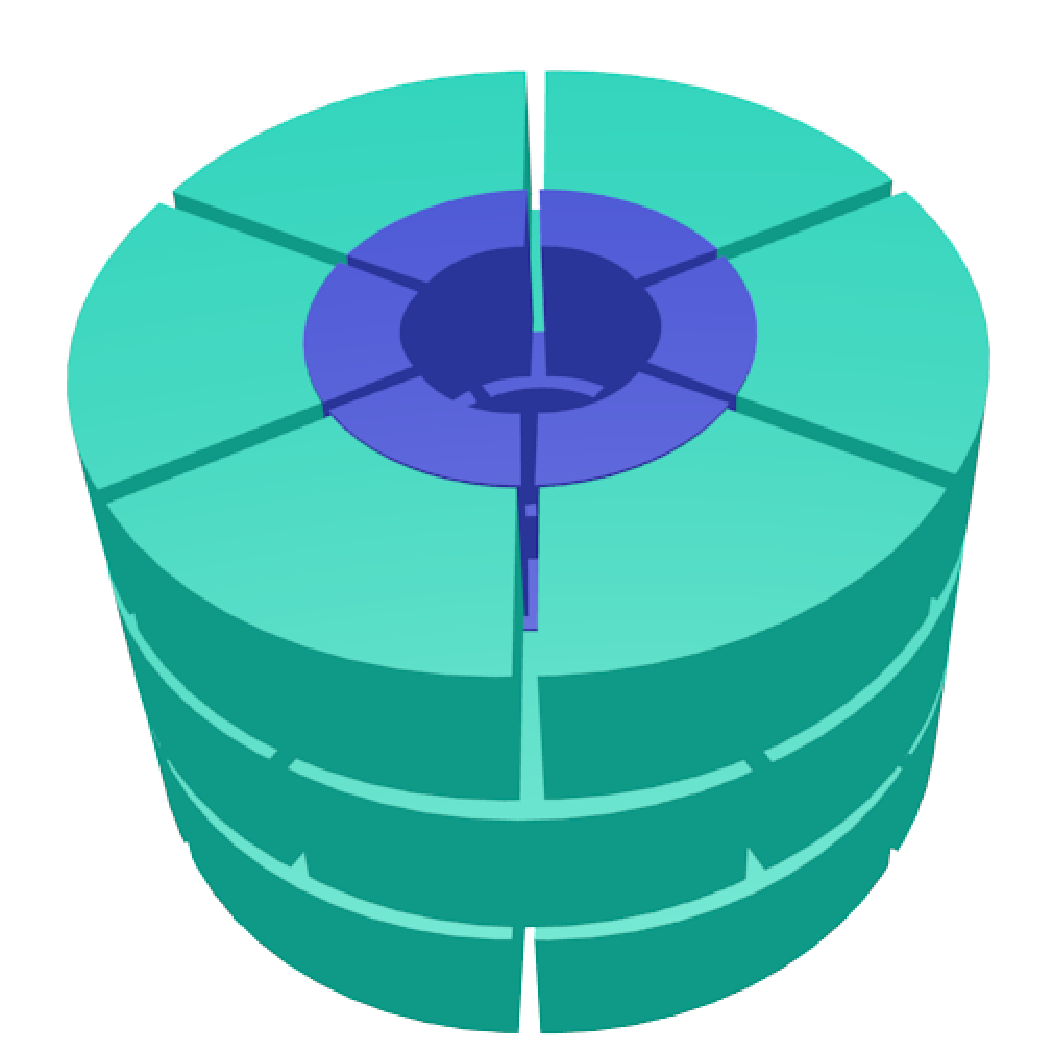
\includegraphics[width=0.6\textwidth]{cartoon_pore.pdf}
		\caption{}~\label{fig:undetailed_pore}
	\end{subfigure}
	\begin{subfigure}{0.45\linewidth}
		\centering
		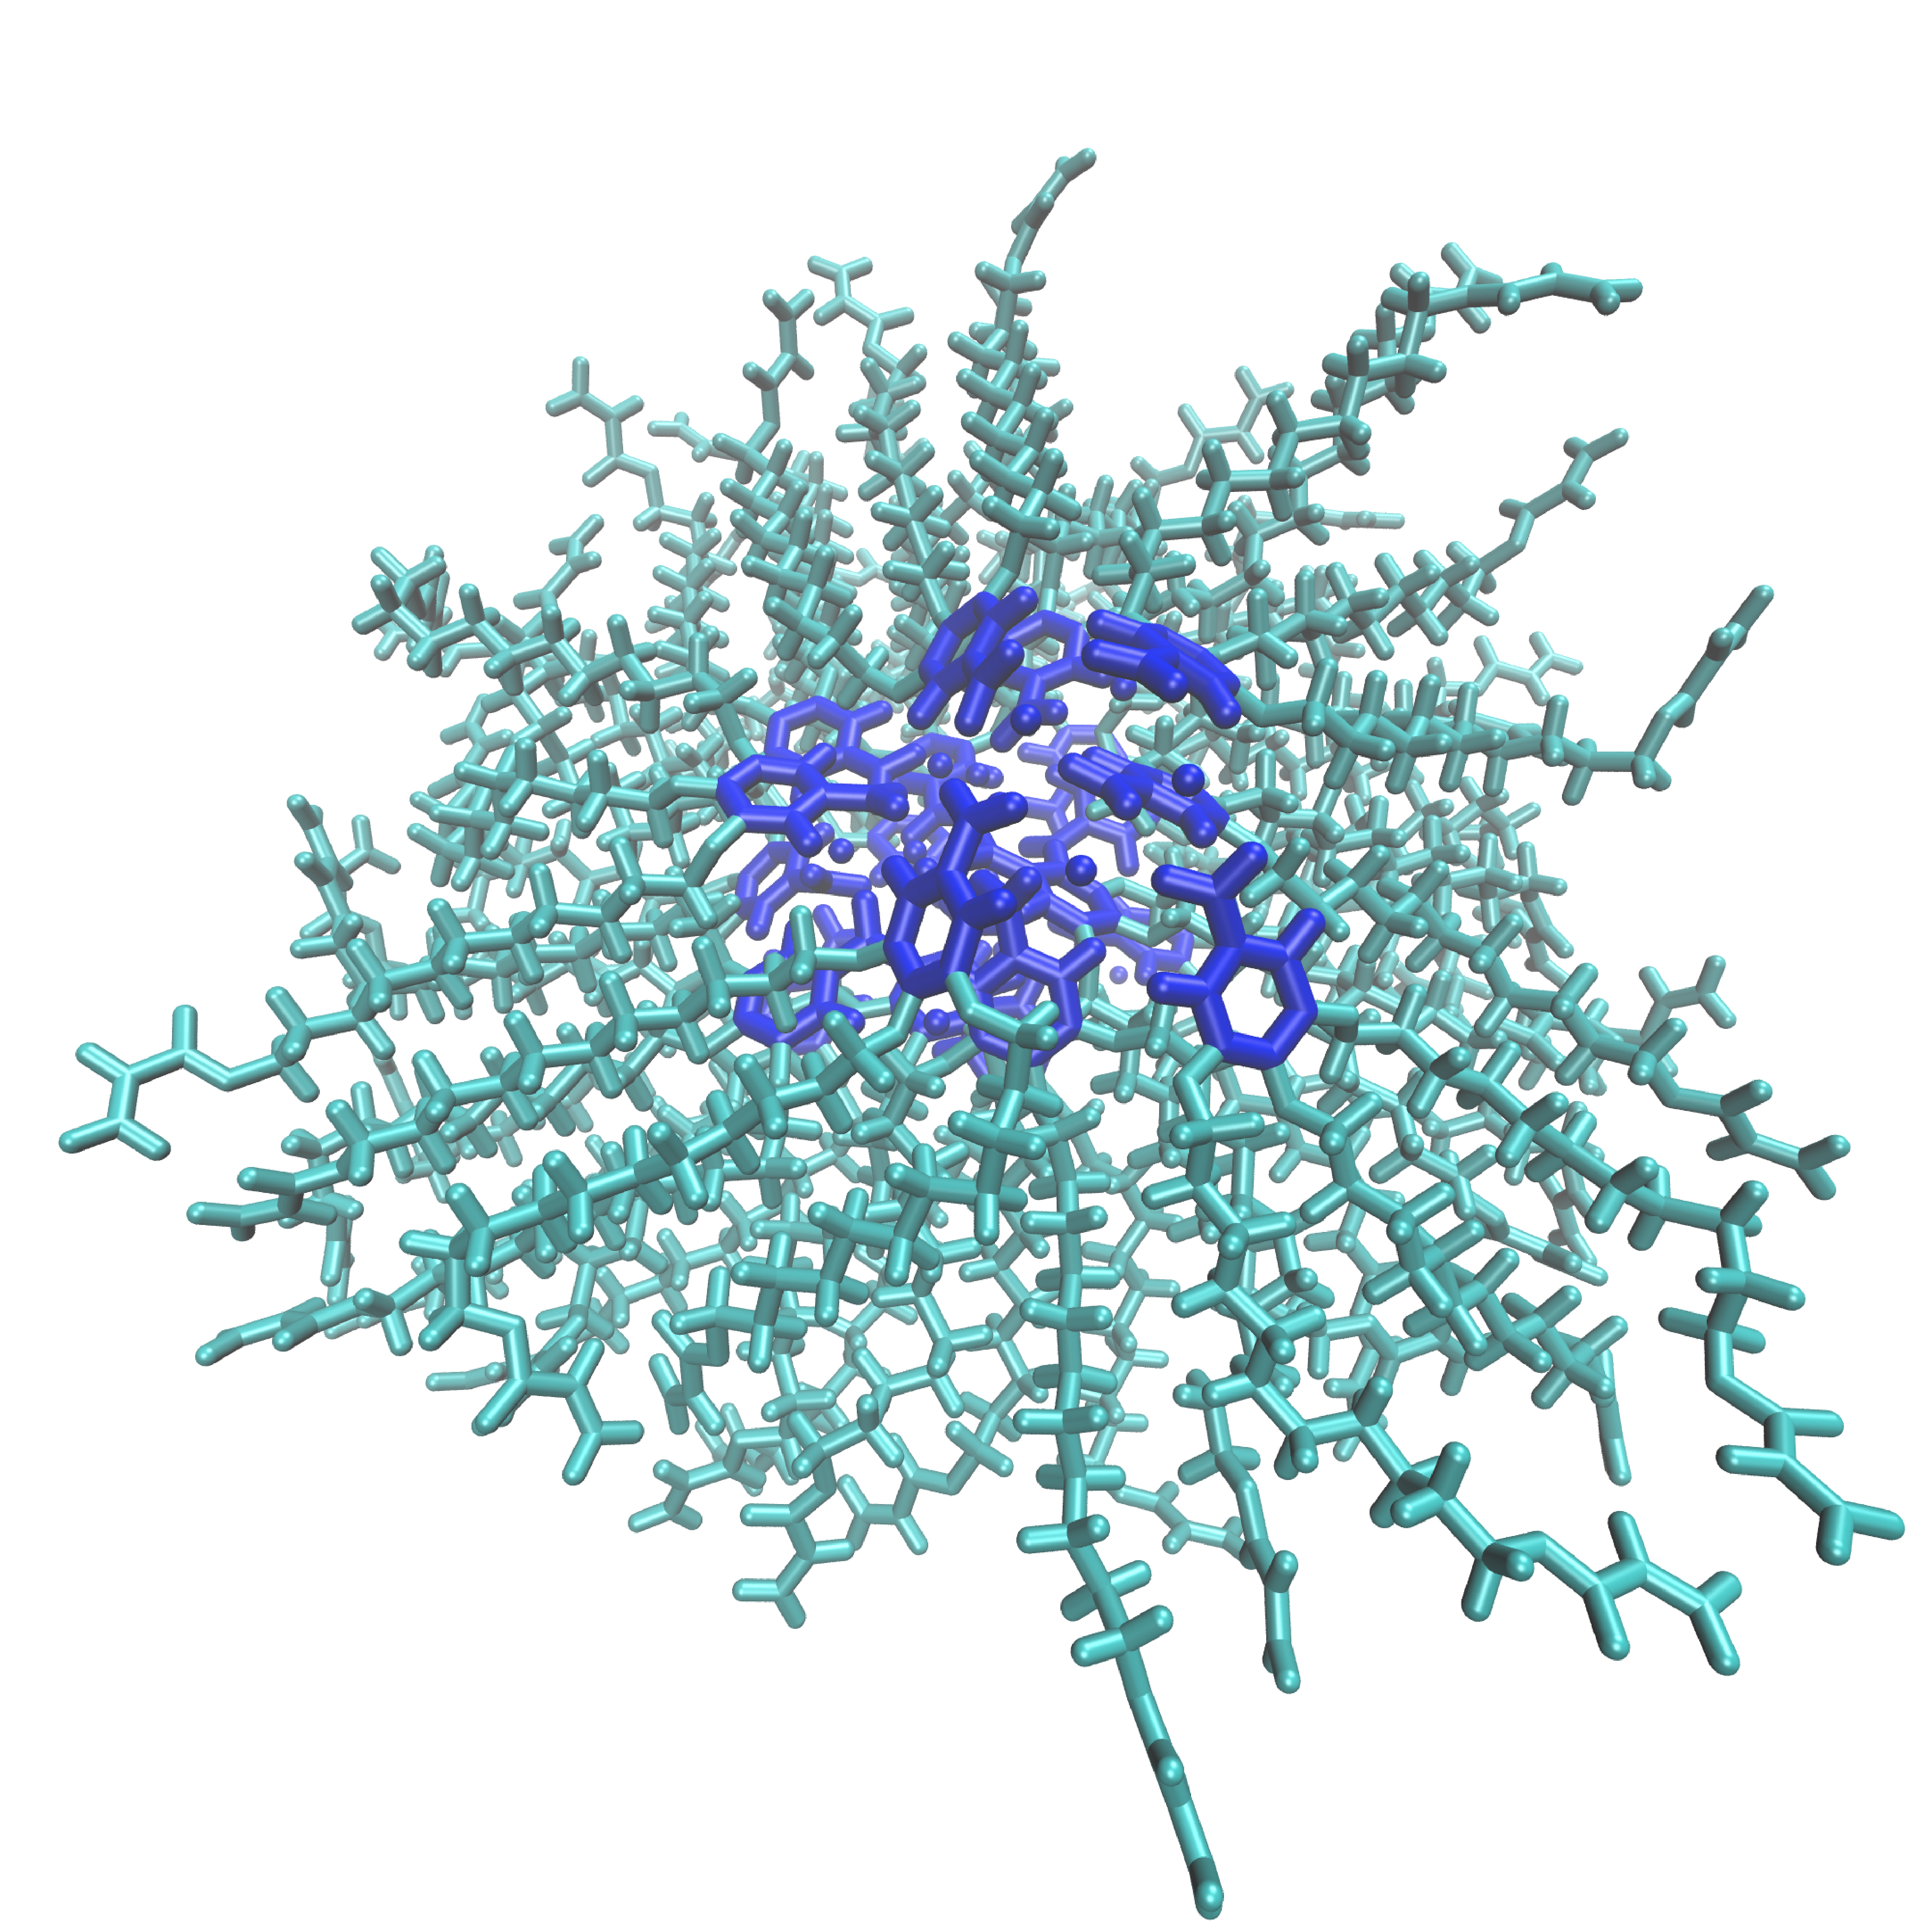
\includegraphics[width=0.6\textwidth]{detailed_pore.pdf}
		\caption{}~\label{fig:detailed_pore}
	\end{subfigure} 
    \caption{(a) Previous understanding of the LLC pores are essentially speculations 
    based on limited chemical and experimental data. (b) We use detailed molecular 
    modeling in this paper in order to appropriately model the pore's complex architecture,
    which is crucial to understanding the mechanism of solute transport. In both 
    pictures, the head group region is colored blue and the tail region is colored cyan.}~\label{fig:detail}
  \end{figure}

  Although the Q\textsubscript{I} phase shows the most promise for
  practical applications, the focus of this work will be on the H\textsubscript{II}
  phase.
  \begin{itemize}
    \item The H\textsubscript{II} phase is an easier to geometry to model
    and analyze.
    \item We also have detailed structural data which is necessary for validating
    our model.
    \item All of the analysis techniques we use can be equally adapted to
    the more complicated Q\textsubscript{I} phase geometry.
  \end{itemize}
  
  There are few molecular simulation studies which study structure and transport
  in LLC systems.
  \begin{itemize}
    \item Mondal et al. used MD simulations to study the self assembly of gemini 
    surfactants and observed the formation of H\textsubscript{II} and Q\textsubscript{I}
    phases depending on water content.\cite{mondal_self-assembly_2013}
    \item Mantha and Yethiraj as well as Roy et al. studied the dynamics of confined 
    water in these systems and showed orders of magnitude differences in their motion
    dependent on system geometry.~\cite{mantha_dynamics_2016,roy_water_2016}
    \item Jackson et al. as well as Mantha et al. have combined experiment with simulation
    in order to show how the choice of monomer head group counterion regulate water 
    dynamics.~\cite{jackson_ion-specific_2018,mantha_counterion-regulated_2018}
    \item Sakamoto et al. and Nada et al. observed the dynamics of water molecules
    and ions and hypothesized transport mechanisms in a simplified model of an LLC
    nanopore.~\cite{sakamoto_development_2018,nada_transport_2020}
  \end{itemize}

  Because there is relatively sparse coverage of these types of simulation systems in 
  the literature, we have built a detailed molecular model from the ground up. There 
  are four primary research questions that we will address in this work.
  \begin{enumerate}
    \item What is the nanoscopic structure?
    	\begin{itemize}
    	  \item Before we can try to understand the molecular mechanisms of solute
    	  transport, we need to ensure that we model the chemical environment
    	  within the nanopores in a way that is consistent with experiment.
    	  \item We use experimental structural data in order to validate our model.
    	\end{itemize}
    \item Which solute-membrane interactions have the greatest influence on transport rates?
    	\begin{itemize}
    	  \item After gaining a detailed picture of the nanopore structure, we can 
    	  feel confident that solutes in this system will experience the same 
    	  interactions which are present in a real system.
    	  \item We create independent systems for each of 20 small polar solutes 
    	  and observe transport mechanisms whose dominance is dependent on
    	  solute chemical functionality.
    	  \item We characterize three different trapping mechanisms which lead
    	  to subdiffusive transport behavior.
    	\end{itemize}
    \item Can we estimate experimentally-relevant macroscopic properties?
    	\begin{itemize}
    	  \item Using our qualitative understanding of the dominant trapping mechanisms,
    	  we develop stochastic time series models which we can use to mimic solute dynamic
    	  behavior on time scales orders of magnitude longer than our simulations. 
    	  \item We attempt to reproduce both quantitative and qualitative solute trajectory
    	  behavior on MD simulation-length timescales.
    	  \item We then show how we can use our most promsiing model in order to connect 
    	  microscopic transport to macroscopic flux and selectivity.
    	\end{itemize}
    \item How can we learn mechanisms with minimal human intervention?  %BJC: i.e. machine learning methods
    	\begin{itemize}
    	  \item Although our stochastic models show great promise, their development 
    	  require some qualitative and quantitative understanding of dominant transport
    	  mechanisms.
    	  \item In the final chapter, we use the infinite hidden Markov model in order
    	  to automatically detect and parameterize a unknown number of hidden dynamical modes
    	  exhibited by solute time series. 
    	  \item This more flexible approach allows us to both infer mechanisms based 
    	  on differences in dynamical behavior and generate stochastic trajectory realizations
    	  which we can use to predict flux and selectivity. 
    	\end{itemize}
  \end{enumerate} 
